%\documentclass[10pt]{beamer}
\documentclass[xcolor={pdftex,dvipsnames,table}]{beamer}

\definecolor{cambridgedarkblue}{HTML}{000000}
\definecolor{cambridgedarkorange}{HTML}{9b0014}

\definecolor{cambridgegreen}{RGB}{88,166,24}
\definecolor{cambridgeorange}{HTML}{9b0014}


\definecolor{redUnipd}{HTML}{9b0014}
\definecolor{grayUnipd}{HTML}{444F51}
\definecolor{myblue}{HTML}{317a9b}
%\definecolor{Black}{RGB}{0,62,114}
\newcommand{\bbf}[1]{\textcolor{black}{\bf #1}}
\newcommand{\rbf}[1]{\textcolor{redUnipd}{ #1}}
\usefonttheme{structurebold}
\usecolortheme[named=myblue]{structure}
\setbeamercolor{structure}{fg=redUnipd}
\setbeamercolor{normal text}{bg=white,fg=grayUnipd}
\setbeamertemplate{itemize items}{$\circ$}
%\textopenbullet
%\usepackage{marvosym}
%\setbeamertemplate{itemize items}{$\Neutral$}

\usepackage{pgfpages}
\pgfpagesuselayout{resize to}[a4paper, 
                                border shrink=1.5cm,
                                landscape]

\usepackage[T1]{fontenc}
%
\usepackage[english]{babel}
\usepackage{graphicx}
\usepackage{booktabs}
\usepackage{latexsym}
\usepackage{subfigure}
\usefonttheme{professionalfonts}
%\usepackage{enumitem}
\usepackage{amsmath,amssymb}
\usepackage[latin1]{inputenc}
%\setbeamercovered{dynamic}
\usepackage{Sweave}
\usepackage[english]{babel}
\usepackage{tikz,comment,amssymb}
\usetikzlibrary{shapes}

\newcommand{\bb}[1]{\begin{block}{#1}}
\newcommand{\eb}{\end{block}}
\newcommand{\bi}{\begin {itemize}}
\newcommand{\ei}{\end{itemize}}
\newcommand{\be}{\begin {enumerate}}
\newcommand{\ee}{\end{enumerate}}
\linespread{1.05}

\newcommand{\bfr}[1]{\begin{frame} \frametitle{#1}}

\AtBeginSection[] {
  \begin{frame}<beamer>
    \frametitle{Outline}
    \tableofcontents[currentsection]
  \end{frame}
}


\title[]{The Labyrinth of Multiple Testing: how to avoid the pitfall of false positives}
\subtitle{12th SISMEC National Congress 2023}
\author[\hspace{5cm}]{Livio Finos and Angela Andreella}
\date{}
% \date{A.A. 2015/2016 }
%\logo{
\includegraphics[scale=.05]{figures/logoUnipd.jpg}}

\begin{document}

\begin{frame}
  \titlepage
\end{frame}

\begin{frame}
\frametitle{American Statistical Association's\\
Ethical Guidelines for Statistical Practice}

% \begin{tabular}{l|l}
Recognize that any frequentist %& $\mathcal{H}=\{A\}$ \\ 
statistical test has a random %&decision rule: reject $A$ if $p_{A}\leq \alpha$\\ 
chance of indicating significance %&$\Pr(p_A\leq \alpha) \leq \alpha$ when $A$ true \\  
when it is not really present. %& (probability of type I error)\\ 
% &\\
\bigskip

Selecting the one ``significant'' % & $\mathcal{H}=\{A, B, C,D\}$ \\
result from a multiplicity of parallel  %& $p_{\min}=\min(p_A,p_B,p_C,p_D)$ \\
tests poses a grave risk of an  %& $\Pr(p_{\min}\leq \alpha)\leq 4\alpha$ when all true \\
incorrect conclusion.   %& (probability of at least one type I error) \\
% &\\
\bigskip

Failure to disclose the full extent % & \\% \\
of tests and their results in such  %&  \\
a case would be highly misleading %& \\
% \end{tabular}
\pause

\bigskip
e.g. VaxGen's AIDSVAX trial \ldots
\end{frame}

%%%%%%%%%%%%%%%%%%%%%%%%%%%%%%%%%%%%%%%%%%%%%%%%%%%%%%%%%%%%%%%%%%%%%%%%%%%%%%%%%%%%%%%%%%%%%%%%%%%%%%
\subsection{}
\begin{frame}
\frametitle{VaxGen's AIDSVAX trial?}


VaxGen announced the results of the first-ever efficacy trial of an AIDS vaccine on 24 February 2003:

\bigskip

%the vaccine failed to prevent HIV infection (primary endpoint):

the vaccine prevent HIV infection?

\bigskip


\begin{tikzpicture}
\node at (0,0.25) {\small{All subjects}};
\node at (2,1) {\small{Total}};
\node at (3.2,1) {\small{Infected}};
\draw (-.8,0.8) -- (3.8,0.8);
\node[text=cambridgegreen]  at (2,0.5) {\small{1679}};
\node[text=cambridgegreen]  at (3.2,0.5) {\small{96}};
\node[text=cambridgeorange]  at (2,0) {\small{3330}};
\node[text=cambridgeorange]  at (3.2,0) {\small{191}};
\draw (-.8,-0.3) -- (3.8,-0.3);
\draw[fill=cambridgegreen] (4,0.3) rectangle +(1.16,0.4);
\draw[fill=cambridgeorange] (4,-0.2) rectangle +(1.14,0.4);
\node[text=cambridgegreen]  at (5.7,0.5) {\small{5.8\%}};
\node[text=cambridgeorange]  at (5.7,0) {\small{5.7\%}};
\node[text=cambridgegreen]  at (8,0.5) {\small{PLACEBO}};
\node[text=cambridgeorange]  at (8,0) {\small{VACCINE}};
\end{tikzpicture}


\bigskip


\emph{"We saw absolutely no difference between the vaccine and placebo groups. Everyone was pretty depressed."}

\bigskip

but the next day...

\end{frame}
%%%%%%%%%%%%%%%%%%%%%%%%%%%%%%%%%%%%%%%%%%%%%%%%%%%%%%%%%%%%%%%%%%%%%%%%%%%%%%%%%%%%%%%%%%%%%%%%%%%%%%
\subsection{}
\begin{frame}
\frametitle{VaxGen's AIDSVAX trial}

...by broking the data down into racial groups -- which they say was part of the original design -- the vaccine appeared to have worked in blacks:

%they broke the data down into racial groups, the vaccine appeared to have worked in blacks:

\bigskip

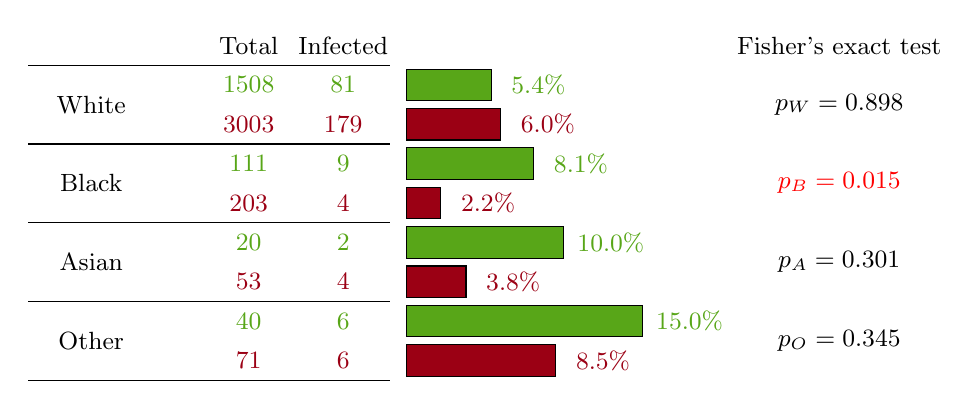
\begin{tikzpicture}
\node  at (9.5,0.25) {\small{$p_W = 0.898$}};
\node[text=red]  at (9.5,-0.75) {\small{$p_B = 0.015$}};
\node  at (9.5,-1.75) {\small{$p_A = 0.301$}};
\node  at (9.5,-2.75) {\small{$p_O = 0.345$}};

\node at (9.5,1) {\small{Fisher's exact test}};
\node at (0,0.25) {\small{White}};
\node at (2,1) {\small{Total}};
\node at (3.2,1) {\small{Infected}};
\draw (-.8,0.75) -- (3.8,0.75);
\node[text=cambridgegreen]  at (2,0.5) {\small{1508}};
\node[text=cambridgegreen]  at (3.2,0.5) {\small{81}};
\node[text=cambridgeorange]  at (2,0) {\small{3003}};
\node[text=cambridgeorange]  at (3.2,0) {\small{179}};
\draw (-.8,-0.25) -- (3.8,-0.25);
\node[text=cambridgegreen]  at (2,-0.5) {\small{111}};
\node[text=cambridgegreen]  at (3.2,-0.5) {\small{9}};
\node[text=cambridgeorange]  at (2,-1) {\small{203}};
\node[text=cambridgeorange]  at (3.2,-1) {\small{4}};
\draw (-.8,-1.25) -- (3.8,-1.25);
\node[text=cambridgegreen]  at (2,-1.5) {\small{20}};
\node[text=cambridgegreen]  at (3.2,-1.5) {\small{2}};
\node[text=cambridgeorange]  at (2,-2) {\small{53}};
\node[text=cambridgeorange]  at (3.2,-2) {\small{4}};
\draw (-.8,-2.25) -- (3.8,-2.25);
\node[text=cambridgegreen]  at (2,-2.5) {\small{40}};
\node[text=cambridgegreen]  at (3.2,-2.5) {\small{6}};
\node[text=cambridgeorange]  at (2,-3) {\small{71}};
\node[text=cambridgeorange]  at (3.2,-3) {\small{6}};
\draw (-.8,-3.25) -- (3.8,-3.25);
\node at (0,-.75) {\small{Black}};
\node at (0,-1.75) {\small{Asian}};
\node at (0,-2.75) {\small{Other}};
\draw[fill=cambridgegreen] (4,0.3) rectangle +(1.08,0.4);
\draw[fill=cambridgeorange] (4,-0.2) rectangle +(1.2,0.4);
\node[text=cambridgegreen]  at (5.68,0.5) {\small{5.4\%}};
\node[text=cambridgeorange]  at (5.8,0) {\small{6.0\%}};
\draw[fill=cambridgegreen] (4,-0.7) rectangle +(1.62,0.4);
\draw[fill=cambridgeorange] (4,-1.2) rectangle +(0.44,0.4);
\node[text=cambridgegreen]  at (6.22,-.5) {\small{8.1\%}};
\node[text=cambridgeorange]  at (5.04,-1) {\small{2.2\%}};
\draw[fill=cambridgegreen] (4,-1.7) rectangle +(2,0.4);
\draw[fill=cambridgeorange] (4,-2.2) rectangle +(0.76,0.4);
\node[text=cambridgegreen]  at (6.6,-1.5) {\small{10.0\%}};
\node[text=cambridgeorange]  at (5.36,-2) {\small{3.8\%}};
\draw[fill=cambridgegreen] (4,-2.7) rectangle +(3,0.4);
\draw[fill=cambridgeorange] (4,-3.2) rectangle +(1.9,0.4);
\node[text=cambridgegreen]  at (7.6,-2.5) {\small{15.0\%}};
\node[text=cambridgeorange]  at (6.5,-3) {\small{8.5\%}};
\end{tikzpicture}

\bigskip

\emph{"The numbers were small, which concerned us, but the result was highly statistically significant. They were pretty incredible results."}

\end{frame}
%%%%%%%%%%%%%%%%%%%%%%%%%%%%%%%%%%%%%%%%%%%%%%%%%%%%%%%%%%%%%%%%%%%%%%%%%%%%%%%%%%%%%%%%%%%%%%%%%%%%%%

\subsection{}
\begin{frame}
\frametitle{Criticisms}

\begin{enumerate}
\item \textcolor{cambridgedarkorange}{\textbf{failure to account for multiplicity}}

\bigskip 

\emph{"The p-values were not adjusted.''}
% 
% \bigskip
% 
% \textcolor{cambridgedarkorange}{Decision rule:} reject $H\in \mathcal{H}$ if $p_H\leq \alpha^{\mathrm{adj}}$\\
% \textcolor{cambridgedarkorange}{Familywise Error:} $\mathrm{FWE}=\Pr(\mathrm{at\,\,least\,\,one\,\,type\,\,I\,\,error})$
% 
% \begin{eqnarray*}
% \mathrm{FWE} =  1-(1-\alpha^{\mathrm{adj}})^{4} = 
% \left\{  \begin{array}{ll}
%     0.187 & \mathrm{if\,\,} \alpha^{\mathrm{adj}}=0.05\\ 
%     0.05 & \mathrm{if\,\,} \alpha^{\mathrm{adj}}=0.0127\\ 
%   \end{array}\right.
% \end{eqnarray*}
% when all null hypotheses are true


\bigskip 

\item \textcolor{cambridgedarkorange}{\textbf{selective reporting (data snooping)}}

\bigskip 

\emph{"It's all murky because it's all post hoc analysis. They might as well do a subgroup analysis based on signs of the zodiac."}

\bigskip

If you torture your data long enough, they will confess you whatever you want to hear!
\end{enumerate}

\end{frame}
%%%%%%%%%%%%%%%%%%%%%%%%%%%%%%%%%%%%%%%%%%%%%%%%%%%%%%%%%%%%%%%%%%%%%%%%%%%%%%%%%%%%%%%%%%%%%%%%%%%%%%
\subsection{}
\begin{frame}
\frametitle{Revived interest in multiple testing}


\textcolor{cambridgedarkblue}{\large{``-omics''}}   \\
\scriptsize{e.g. genomics experiments with microarray data: which genes are differentially expressed?}
\smallskip
\smallskip

\textcolor{cambridgedarkblue}{\large{model selection}}\\
\scriptsize{e.g. multiple regression: which coefficients matter?}
\smallskip
\smallskip

\textcolor{cambridgedarkblue}{\large{econometric}}\\
\scriptsize{e.g. comparing several strategies with a benchmark: any better? which ones?}
\smallskip
\smallskip

\textcolor{cambridgedarkblue}{\large{...}}
\smallskip
\smallskip


\begin{block}{\Large \textbf{clinical trials}}
\begin{columns}[t]
\column{0.45\textwidth}
\normalsize{
\textcolor{cambridgedarkorange}{sources of multiplicity}
\begin{itemize}
\item multiple endpoints
\item several treatments
\item multiple time points
\item subgroup analysis
\item interim analysis
\item $\ldots$
\end{itemize}}

\column{0.45\textwidth}
\normalsize{
\textcolor{cambridgedarkorange}{regulatory guidelines}
\begin{itemize}
\item statistical principles for clinical trials (ICH E9)
\item points
to consider on multiplicity issues in clinical
trials (EMEA)
\item $\ldots$
\end{itemize}}
\end{columns}
\end{block}



\end{frame}

\subsection{}
\begin{frame}
\frametitle{Verifica di Ipotesi, Un solo test}

\rbf{Due Ipotesi a confronto}

\begin{itemize}
\item $H_0$: due gruppi sono Uguali, nessuna relazione tra $X$ e $Y$, 
\item $H_1$: due gruppi sono Diversi, there is relazione tra $X$ e $Y$,
\end{itemize}
Ogni test produce un p-value $p$, \\  se $p\leq .05$ ($\alpha=.05$) rifiuto $H_0$ (e propendo per $H_1$)
\end{frame}

\subsection{}
\begin{frame}
\frametitle{Errori}

\begin{itemize}
\item \bbf{Tipo I} (falso positivo): Rifiuto $H_0$ quando \`e Vera \\
$P(Errore\ Tipo\ I)=P(p\leq .05 | H_0)=.05$
\item \bbf{Tipo II} (falso negativo): Non Rifiuto $H_0$ quando \`e Falsa \\
$P(Errore\ Tipo\ II)=P(p> .05 | H_1)$\\
\bbf{Potenza}: 
\begin{eqnarray}\nonumber P(p\leq .05 | H_1)&=& 1-P(p>.05 | H_1)\\ \nonumber &=& 1-P(Errore\ tipo\ II) 
\end{eqnarray}
\end{itemize}
\end{frame}

\subsection{}
\begin{frame}
\frametitle{Importanza asimmetrica degli errori}

Controlliamo la $P(Errore\ tipo\ I)$ (es $\leq .05$)\\
e cerchiamo il test con massima Potenza (minimo $Errore\ tipo\ II$)
\bigskip

\`E importante ricordare che
\bi
\item[-] un p-value significativo ($p\leq\alpha$) ci autorizza a pensare che sia vera $H_1$, mentre
\item[-] un p-value non significativo ($p>\alpha$) NON ci autorizza a pensare che sia vera $H_0$, semplicemente non abbiamo abbastanza evidenza per rifiutarla.
\ei
\end{frame}

\subsection{}
\begin{frame}
\frametitle{Errori di Tipo I:}

$P(p\leq .05 | H_0=\textrm{i 2 gruppi sono Uguali})=?$\\
Supponiamo $H_0: \mu_1-\mu_2=0$ e $H_1: \mu_1-\mu_2<0$\\
statistica test $T=\frac{\bar{x}_1-\bar{x}_2}{\hat{\sigma}}$ ( $\hat{\sigma}$ stima della dev std di $\bar{x}_1-\bar{x}_2$)\\
sotto $H_0$: $T\sim t_{n_1+n_2-2}$, allora\\
% \begin{columns}[t,onlytextwidth]
% \begin{column}{width=0.6\textwidth}
\begin{eqnarray*}
P(T\leq t_\alpha | H_0) =\alpha \ \forall \alpha\\
P(F(T)\leq F(t_\alpha) | H_0) =\alpha \ \forall \alpha\\
P(P \leq \alpha | H_0) =\alpha \ \forall \alpha
\end{eqnarray*}
ne consegue che $P\sim U(0,1)$
% \end{column}
% \begin{column}{width=0.4\textwidth}
\begin{center}
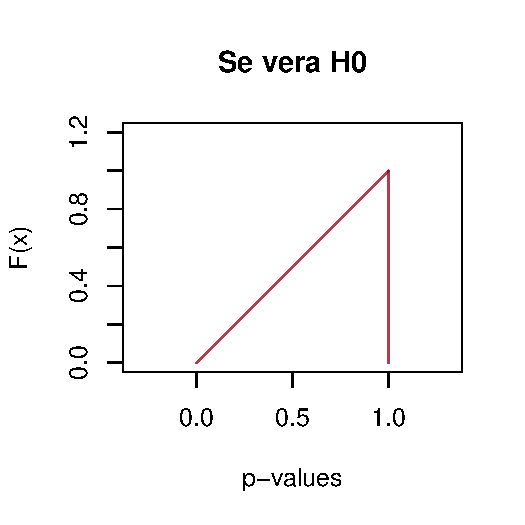
\includegraphics[width=0.3\textwidth]{plaatjes/cdf_uniform}      
\end{center}
% \end{column}
% \end{columns}

\end{frame}

\subsection{}
\begin{frame}
\frametitle{Errori di Tipo I:}

\begin{overprint}
\only<1> {Sotto $H_0$ il p-value \`e una variabile aleatoria uniforme $U(0,1)$}
\only<2> {Errore di I tipo: $P(p\leq .05 |H_0)=.05$} % (o almeno $\leq .05$)}
\end{overprint} 
\begin{overprint} 
\onslide<1> \centerline{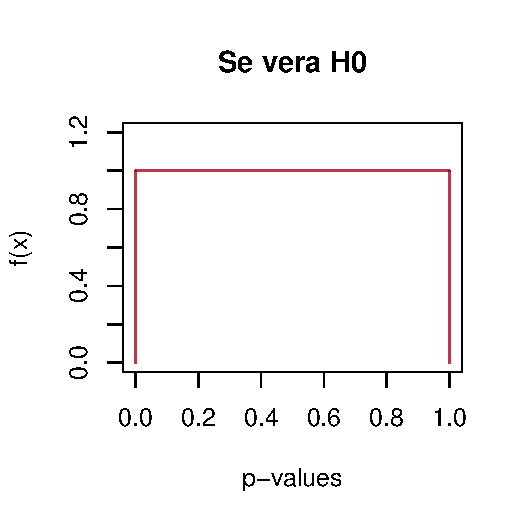
\includegraphics[width=8cm]{plaatjes/uniform1}}
\onslide<2> \centerline{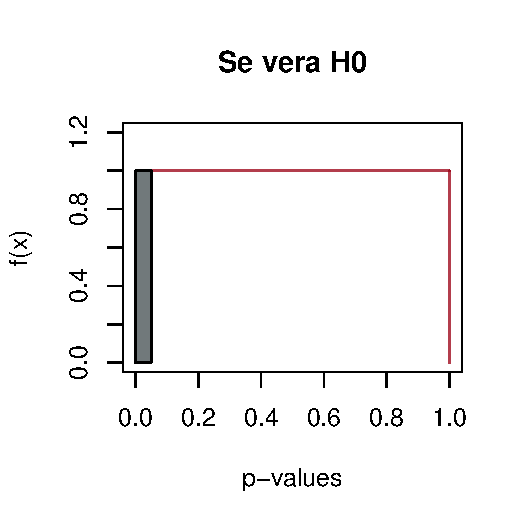
\includegraphics[width=8cm]{plaatjes/uniform2}}
\end{overprint} 
\end{frame}

\subsection{}
\begin{frame}
\frametitle{Potenza}

$P(p\leq .05 | H_1=2\ gruppi\ Diversi)$
\begin{overprint}
% \onslide<7> ad es: $Potenza: P(p\leq 0.05 | H_1)=0.74$
\only<1> {\small Sotto $H_1$ il p-value \`e stocasticamente inferiore ad una variabile aleatoria uniforme $U(0,1)$ (Non distorsione del test)}
\onslide<2> {Sotto $H_1$ $P(p\leq .05 |H_1)>.05$, nel nostro caso $= .74$\\ }
\end{overprint}
\begin{overprint} 
\onslide<1> \centerline{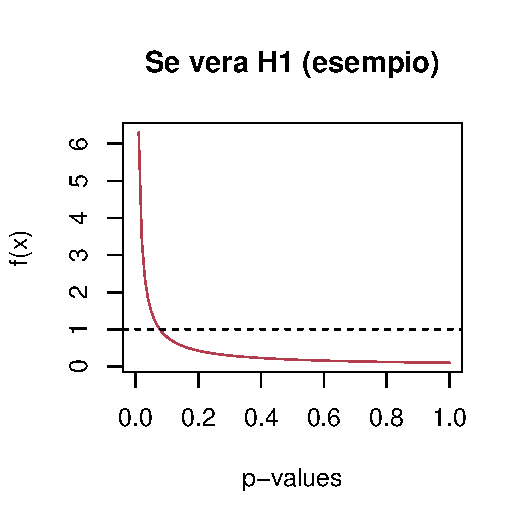
\includegraphics[width=7cm]{plaatjes/beta1}}
\onslide<2> \centerline{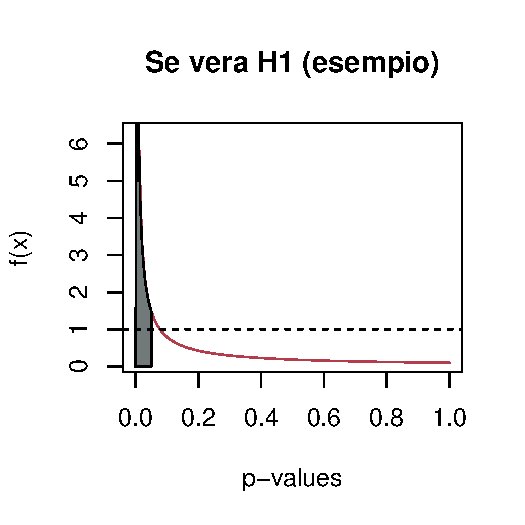
\includegraphics[width=7cm]{plaatjes/beta2}}
\end{overprint} 
\end{frame}

\subsection{}
\begin{frame}
\frametitle{Errori di Tipo I, Due Test (indipendenti)}

Propabilit\`a di ALMENO un (falso) rifiuto?\\
$P(p_1\leq .05 \cup p_2\leq .05 | H_0)= .05+.05-(.05\cdot .05)=1-(1-.05)^2=.0975=1-(1-\alpha)^2$

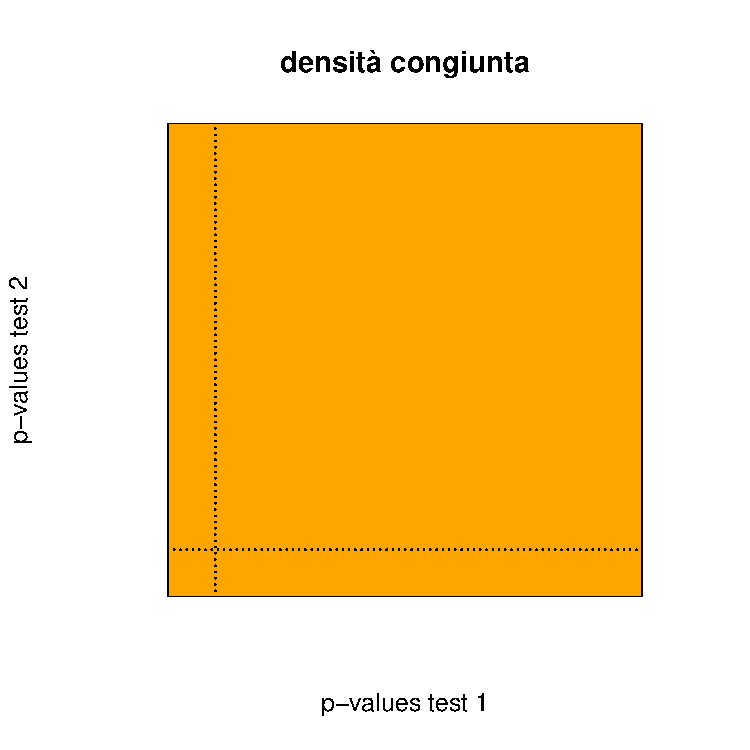
\includegraphics[scale=.5]{plaatjes/bivaH0indep}
\end{frame}

\subsection{}
\begin{frame}
\frametitle{Probabilit\`a di falsi rifiuti}

\bb{$m$ p-value indipendenti}
Se rifiuto l'ipotesi quando $p\leq \alpha$
\eb
\bb{Probabilit\`a ALMENO un falso rifiuto}
$P = 1- (1-\alpha)^m$
\eb

\pause
\bigskip
Questo diventa ben presto un problema, se $m$ diventa grande ...

\end{frame}

\subsection{}
\begin{frame}
\frametitle{Errori di Tipo I in funzione del numero di test ($m$)}

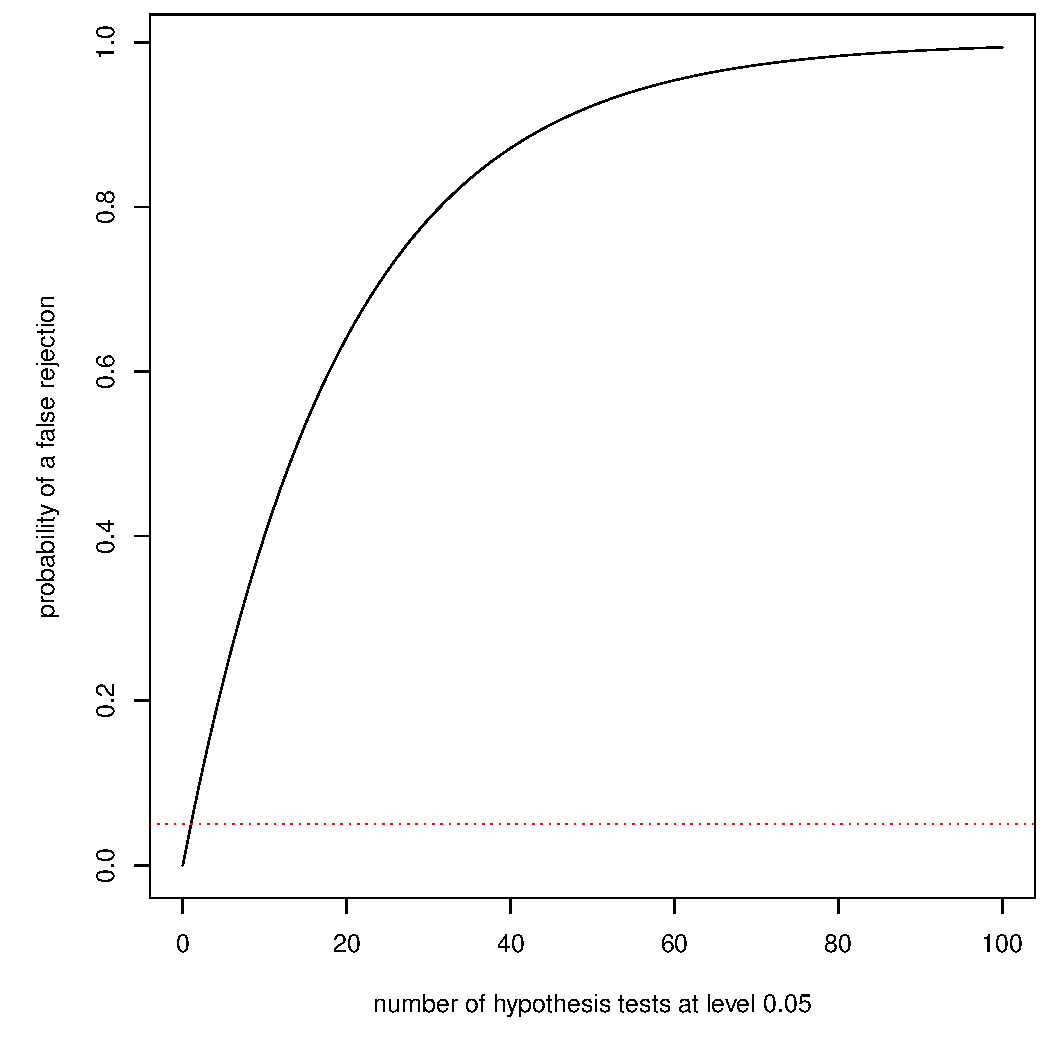
\includegraphics[scale=.3]{plaatjes/typeI}
\end{frame}


\subsection{}
\begin{frame}
\frametitle{Type I error}
\bb{Come definire l'errore di tipo I quando ci sono molte ipotesi?}
\eb
\bb{Quali procedure controllano questo errore?}
\eb
\end{frame}

\end{document}


